\let\negmedspace\undefined
\let\negthickspace\undefined
\documentclass[journal]{IEEEtran}
\usepackage[a5paper, margin=10mm, onecolumn]{geometry}
%\usepackage{lmodern} % Ensure lmodern is loaded for pdflatex
\usepackage{tfrupee} % Include tfrupee package

\setlength{\headheight}{1cm} % Set the height of the header box
\setlength{\headsep}{0mm}     % Set the distance between the header box and the top of the text

\usepackage{gvv-book}
\usepackage{gvv}
\usepackage{cite}
\usepackage{amsmath,amssymb,amsfonts,amsthm}
\usepackage{algorithmic}
\usepackage{graphicx}
\usepackage{textcomp}
\usepackage{xcolor}
\usepackage{txfonts}
\usepackage{listings}
\usepackage{enumitem}
\usepackage{mathtools}
\usepackage{gensymb}
\usepackage{comment}
\usepackage[breaklinks=true]{hyperref}
\usepackage{tkz-euclide} 
\usepackage{listings}
% \usepackage{gvv}                                        
\def\inputGnumericTable{}                                 
\usepackage[latin1]{inputenc}                                
\usepackage{color}                                            
\usepackage{array}                                            
\usepackage{longtable}                                       
\usepackage{calc}                                             
\usepackage{multirow}                                         
\usepackage{hhline}                                           
\usepackage{ifthen}                                           
\usepackage{lscape}
\begin{document}

\bibliographystyle{IEEEtran}
\vspace{3cm}

\title{1.10.7}
\author{EE24BTECH11037 - Manognya Kundarapu
}
% \maketitle
% \newpage
% \bigskip
{\let\newpage\relax\maketitle}

\renewcommand{\thefigure}{\theenumi}
\renewcommand{\thetable}{\theenumi}
\setlength{\intextsep}{10pt} % Space between text and floats


\numberwithin{equation}{enumi}
\numberwithin{figure}{enumi}
\renewcommand{\thetable}{\theenumi}


\textbf{Question}:\\
The vector in the direction of vector $\hat{i} - 2\hat{j} + 2\hat{k}$ that has a magnitude $9$ is
\begin{enumerate}
\item $\hat{i} - 2\hat{j} + 2\hat{k}$
\item $\hat{i} - 2\hat{j}$
\item $3\brak{\hat{i} - 2\hat{j} + 2\hat{k}}$
\item $9\brak{\hat{i} - 2\hat{j} + 2\hat{k}}$
\end{enumerate}
\solution
\begin{table}[ht!]    
  \centering
  \begin{tabular}[12pt]{ |c| c|}
    \hline
    Direction vector & $\hat{i} - 2\hat{j} + 2\hat{k}$ \\
    \hline 
    magnitude & $9$\\
    \hline 
    \end{tabular}
  \caption{given information}
  \label{tab10.5.3.9.1}
\end{table}\\
Required vector be $c$ 
$\begin{pmatrix}
1\\
-2\\
2
\end{pmatrix} = \underline{\mathbf{v}}$\\
Given
$\| c\underline{\mathbf{v}} \|$ $= 9$\\
$ \implies \sqrt{9c^2} = 9 $\\
$ \therefore c=3$\\
$ \implies $ Option 3 is correct.

\begin{figure}[h!]
   \centering
   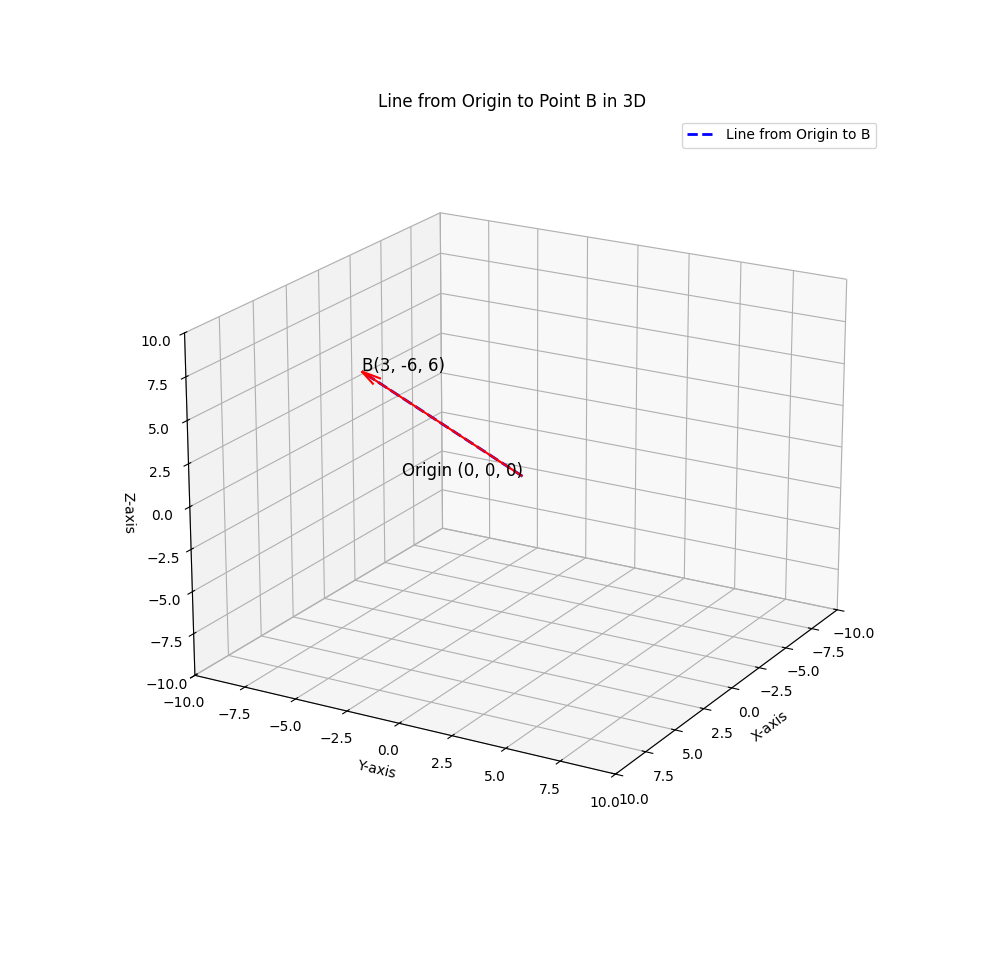
\includegraphics[width=0.7\linewidth]{Figure_1.png}
   \caption{Stem Plot of y\brak{n}}
   \label{stemplot}
\end{figure}
\end{document}  
